\begin{abstract}
\noindent
The object of this study is to provide the information necessary for
prospective participants to make an informed decision about 
cooperating on a `free network' in the area around Lincoln College Preparatory
Academy. \par
In Part I of the study, we give an overview of the motivations, methodologies and
design patterns behind free networks, their component technologies, and potential
applications. In Part II, we explain the architecture and current footprint of the Kansas City
Freedom Network. Finally, in Part III of the study, we examine the feasibility
of extending the KCFN to the
area surrounding Lincoln Prep, propose a plan for doing so, and give estimates
of cost.\par
Our finding is that launching such a network is certainly feasible, and would provide significant
 benefits to the KCPS and its students, neighborhood residents and businesses, and the 
community at large.\par
\end{abstract}

\section{Introduction}\label{Introduction}
\subsection{Network Models -- Proprietary, Private, \& Free}
The vast majority of people think of `The Internet' as a monolith. In
actuality, however, The Internet is made up of some ~40,000 carrier networks,
interoperating via shared protocols, and with the autonomy to run their networks
as they see fit. While some of these networks are state-run or designed for
research and education, the vast majority are `proprietary' networks.
Proprietary networks have many advantages, including large
geographic reach, access to wholesale connectivity markets, and the ability to
peer with other networks. With these advantages, however, come some significant
limitations. Proprietary networks are owned by telecom companies, and their use
comes at a steep cost to the user. Moreover, users have little to no say over
how the network is run, meaning that they are perpetually at the mercy of the
operator to upgrade or troubleshoot the network. \par
At the same time, countless private networks extend connectivity 
into homes and businesses worldwide. While these networks are limited in their
reach, they offer their owners the freedom to decide when, where, and how the network functions.
Home users  establish private networks (generally referred to as Local Area
Networks) for a variety of reasons, including
added security, the ability to serve multiple devices via a single gateway, and
to enable wireless connectivity. In corporate and public sector IT environments, 
private networks (generally referred to as intranets) are used to support a wide 
array of business-critical applications. \par  
Until recently, there was a sharp distinction between proprietary networks and their
private counterparts. Networks were either large, commercial enterprises or
small, private undertakings meant to augment an existing Internet connection.
Over the past few years, however, advances in network technology have led to the
emergence of a new sort of network. These new networks, refered to as `free'
networks, represent a middleground. They are capable of achieving significant
geographic reach and of peering with other networks, yet they also give their
owners the freedom to build, upgrade, and utilize connectivity as they see fit. 
This blend of capabilities and freedoms is achieved by a model in which
ownership is distributed amongst many parties under a common license.\par
Using powerful, low-cost  microwave equipment and the free network model,
communities throughout the world have been able to save money and spur economic
development, while at the same time
working to ensure that none are left without lifeline access. Such networks now
span major cities and entire regions, participate in large Internet Exchange Points
(wholesale markets where carriers exchange traffic), and enable innovative and community-driven 
applications. \par
The basic principle behind free networks is the same principle that has
catapulted the Internet to its profound success - that when networks join
together, the sum is much greater than its parts. In networking theory, this
principle is known as \emph{Metcalf's Law}. \par 
The upshot for individuals and community institutions is that owning part of a
common network is a much better value proposition than owning all of a private
one. In exchange for contributing their resources, participants are
allowed to utilize those resources contributed by others. While contributors
retain complete and total ownership of their infrastructure, they license its
use to other participants in exchange for a reciprocal agreement. This is the
purpose of the \emph{Network Commons License} --- a legal framework for
governing free networks maintained by a global consoritum including The Free
Network Foundation. \par
This framework works particularly well in computer networks, where technical
measures can be used to make sure that participants don't utilize more than
their fair share of the network's resources.
In this way, we can avoid the \emph{tragedy of the commons}
and bolster the long-term sustainability of the network. \par
Yet, technical measures are not enough to guarantee success. In order for the
network to thrive, it is essential that it be coupled with a significant
educational effort. The free network model requires that participants and
prospective participants actually be able to take advantage of the freedom to
expand and improve the network. The skills to do so are easily attainable, but
the fact remains that they must be attained. In the end, the only way to achieve
a sustainable model is for those who use the network to be its primary stewards.\par
Many high-profile municipal networks have failed precisely because individuals
and businesses were not allowed, were not able, or were not willing to make necessary improvements.
To this end, it is critical that the network be built with free and open
technologies, that it be as simple as possible to operate and maintain, and
that community egagement be made a priority at every turn.\par
Using open technologies and providing ample educational opportunities fosters
a highly distributed ownership model. It is this model that gives free networks
their strength --- empowering communities to own their own networks,
\emph{without} requiring outsized commitments of capital, and \emph{with} a
boundless potential for good.

\subsection{Free Network Advantages}
Free networks are more than just the Internet --- they're an opportunity for a new
sort of connectivity, rooted in community. While significantly reducing barriers
to access is certainly one of their primary benefits, they are also designed to
serve as a platform for community media, local applications, and advanced
functionalities. \par
It is important to understand that while free networks can (and should) be
connected to the global Internet, they are first and foremost independent
networks. Aside from the electricity required to run the network equipment (less
than a lightbulb per home), there is no cost for moving data \emph{within} the network.
Because free networks function as a commons, participants can communicate
with one another directly, without ever having to pay an ISP for service.
With this in mind, here are just a few of the potential applications:
\begin{itemize}
\itemsep0em
\item By connecting the network to an Internet Exchange Point or other wholesale
connectivity market, it is possible to provide all those who wish to access the
Internet with significantly less expensive options for getting online. In this
regard, the network essentially functions as an Internet co-op --- by pooling
their purchasing power, participants are able to get much better prices than
they ever could on the retail market.
\item By connecting the network to a school or business intranet, students and
faculty or employees can be granted secure, authenticated access to an
organization's digital resources, including an Internet gateway. 
\item Educational and cultural institutions can easily make content archives and
learning materials available to the community without having to pay for web
hosting. This is especially beneficial when the content is multimedia, 
which requires significant amounts of bandwidth.
\item Network participants can make video and voice calls to one another without
having to pay for cellular or Internet service.
\item Organization of the network by neighborhood and block encourages the
establishment and use of bulletin boards and chatrooms that connect neighbors
and strengthen communities.
\item Youth can learn valuable skills by building and maintaining the
network. These system administration skills are highly sought after by employers. 
The use of free and open tools means that anyone can understand
and improve the network. 
\end{itemize}

\subsection{Wireless Communications}
In Internet-speak `Layer 1' refers to the physical medium used to transmit
information. A variety of Layer 1 technologies exist, such as hybrid-fiber-coax
(Cable), copper (DSL and Ethernet), fiber optics (Active Ethernet), and microwave
(WiFi, Cellular). Most free networks use microwaves as their primary medium, though larger
freenets also make use of copper and fiber optics. Each of these media
has its own set of benefits and drawbacks --- the choice of which to use is
driven by the interplay of geography and economics. It is our opinion that
microwave represents the optimal choice for this project. \par
In large part this is due to the fact that microwave infrastructure is by far
the least expensive to install and maintain. It does not require the
trenching or hanging of cables, nor does it require expensive or proprietary
equipment. Since it first came to the consumer market twenty years ago, the cost
of microwave network capacity has decreased by a factor of more than 1000x. This
trend continues today, with a host of significant advances achieving commercial
viability. \par
At the same time, microwave is not without significant drawbacks. In the United States,
unlicensed microwave communications is restricted to three specific frequency
bands. As more and more WiFi
devices come online, these bands are becoming increasingly congested. Left unchecked and unmanaged,
this interference has the potential to significantly reduce network performance. 
\par
In addition to congestion, it is important to consider the fact that
microwaves are significantly weakened when passing through opaque materials such
as earth, wood, concrete, and steel. While some penetration of these materials
is possible, backbone network links demand a clear path, and
repeaters will be required to cover the insides of buildings.  \par 
Despite these limitations, microwave technology ultimately represents the best
choice of medium due to its long range, small cost, and ease of use. As the
network grows and capacity demands increase microwave links can be reinforced with 
copper, fiber, and advanced wireless technologies such as milimeter-wave and laser.\par
 
\subsection{Free Network Architecture}
The architecture employed by the KCFN was developed by the Free Network
Foundation between 2011 and the present, in collaboration with networking groups from around the
world, including guifi.net, Freifunk, WLAN Slovenia, and Connecting for Good.\par

\subsubsection{Physical Plant}
Before any network devices are powered on,
there is a significant amount of engineering and effort that must go in to making
sure network hardware is safely installed. Here are a few of the best practices in device
installation:
\begin{description}
\item[Cabling] It is important that all outdoor cable installation be done with
UV-rated, shielded ethernet cables. We recommend Ubiquiti ToughCable Carrier
Grade, for its low cost and outstanding durability. Indoor installations should
always use plenum-rated cable, to ensure that cables do not become a health
hazard in case of a fire. We also recommend that all cables be installed out of
the public eye, and out of the public reach. 
\item[Mounting] Devices mounted to the sides of building should be anchored into
masonry or studs, and should be mounted using UFL approved brackets.
Self-tapping screws ease installation, and provide for a secure brace.
\item[Masts] The two primary methods for mast construction are 
hold-offs and non-penetrating roof mounts. Hold-off mounts should be secured in
at least three places, and anchored into masonry. Roof mounts should use UFL
approved bases, dense masonry ballast, and a non-conducting mast, such as EMT
conduit. The weight of the ballast, in ounces, should exceed the wind-bearing
surface area of any antenna elements, in square inches, by a factor of five.
\item[Power Delivery] For safety and ease of installation, we recommend that
power be delivered to all devices using IEEE 802.3 Power-over-Ethernet. In this
way, no electrical cabling has to be installed, and electrical hazards are
significantly curtailed.
\item[Grounding] Any installations that exceed their
surroundings in height should be grounded. This can be achieved by running a
ground wire, or by using grounded RJ-45 ethernet jacks, and cable that has an
integral ground wire, such as Ubiquiti ToughCable.
\item[Gear Security] Gear  such as switches, dedicated
routers, servers, and power distribution units should be located indoors or in a
weather-rated outdoor enclosure. Indoor installations should be placed in a utility
closet or other secure room. 
\end{description}


\subsubsection{Hardware}
Through lab and field testing, we have selected components and developed a suite
of four network devices. All of the hardware employed is readily available,
off-the-shelf equipment, selected for performance, durability, and software
support. We call this suite of devices the `FreedomStack':

\begin{description}
\item[FreedomNode] The node is the smallest of the four devices, and is designed
to connect a single family or small business to the network. For optimum
performance, the node should be located indoors, such that it has a view of the nearest
relay. The suggested hardware for a node costs under \$50. In case a home or
business already has a router, the cost can be reduced to less than \$25.\par
{\bf Technical Details:} The recommended
hardware for a FreedomNode is the Netgear WNDR3800, though any WRT-compatible
dual-band router can be used. By using a dual-band device, the node is able to
connect to the Freedom Network on the 5.8GHz band, while using the 2.4GHz band to
provide access to clients devices such as laptops, tablets, and phones. In this
way, the node functions as a wireless modem, and as a wireless router. For modem
functionality alone, we recommend the TP-Link 703n.

\item[FreedomRelay] The relay is a block-level network anchor. It serves to
connect a group of nodes to the neighborhood-wide network.   Relays should be placed outdoors,
such that they can be seen by as many nodes as possible, and so that they can
see a neighboring relay or tower. The suggested hardware for a relay costs under
\$500. \par
{\bf Technical Details:} The recommended
hardware for a FreedomRelay is a ALIX 2D2 Motherboard with two Ubiquiti SR71-15
SuperRange radio modules, four 5GHz 8dBi omni antennae, MMXC to SMA feed cables,
outdoor enclosure, passive Power-over-Ethernet adapter and associated
mouting hardware.  The use of a dual-radio setup enables the relay 
to perform as a full duplex device, avoiding the need for a single radio to split
its time between receive and transmit cycles. The relays and nodes in any given
neighborhood form a mesh network, meaning that devices can move around or power
off, and the rest of the network will adapt and continue to function. The use of
duplex devices is critical for the performance of the mesh.

\item[FreedomTower] The tower is a neighborhood-level network hub. It
acts as a bridge between a neighborhood network and the city-wide network of
towers. Towers must be located on roofs or hilltops with line of sight to
at least two other towers.
 The baseline cost for a tower is roughly \$1300. \par
{\bf Techincal Details:} The recommended hardware for a FreedomTower is two Ubiquiti Rocket M5's equipped
with 30 dBi dish antennae, three Rocket M5's equipped with 16 dBi 120-degree
sector antennae, and a Ubiquiti ToughSwitch8-Pro. 

\item[FreedomLink] The link is intended to serve as a city-wide 
Internet gateway, content server, network controller, or all of the above. Links must be placed in a
datacenter environment, with roof access for the radio gear and line of sight to
at least two towers. While the suggested hardware for a link costs \$3000, link
operation requires an ongoing capital expenditure of at least \$250/month. \par
{\bf Technical Details:} The 
recommended hardware for a FreedomLink is two Ubiquiti Rocket M5's equipped with 30 dBi dish
antennae, four Dell PowerEdge 2950 rackmount servers, and one Cisco Catalyst
WS-C2960S-24TS-S 24-port 10/100/1000 switch. 
\end{description}

\subsubsection{Firmware}
Of the devices listed above, the majority are classified as `embedded
devices' --- low-power computers responsible for a very specific task. These
particular devices are designed to establish wireless links and make decisions
about network routing. In order to function, they require an operating system
for embedded systems, otherwise known as a 'firmware'. \par
In addition to their performance and reliability, the selected hardware was
chosen because it is capable of running OpenWRT, a significantly stripped down
version of the GNU/Linux operating system that powers most web servers. Free
networks run on free software, because access to the source code makes it
possible to know exactly what is going on inside the machine, and to
make any modifications one desires. \par 
OpenWRT comes in many varieties, each with its own set of features. The Kansas
City Freedom Network uses a customized version of \emph{quick mesh project} or
qmp. qmp is mesh network firmware that leverages recent advances in network
routing and management, and is maintained by The guifi.net Foundation. In
addition to the basic utility of OpenWRT, it has the following advanced
functionalities:

\begin{description}
\item[Address Management] IP address management is handled automatically,
without user or administrator intervention. The default behaviour is to assign
each device a block of addresses capable of supporting 255 clients. \par 
{\bf Techincal Details:} During the device initialization
process, a unique address is generated by cryptographically hashing the MAC
address of the primary network adapter. The chosen hash function is the CRC-16
cipher. 
\item[Routing] The routing protocol employed by qmp is BMX6, developed
by Axel Neumann of Freifunk Berlin. The protocol is used to dynamically
determine the best path for traffic.
\par
{\bf Technical Details:}  BMX6 is an IPv6 native, distance-vector protocol.
It is designed to automatically respond not just to changes in the network, but to 
the actual quality of the links between devices. BMX6 has excellent loop
avoidance and route convergence properties, but perhaps its greatest strength is
extremely low overhead, especially when compared to other mesh systems.
\item[Instrumentation \& Management] qmp includes tools for collecting
information on usage and device status through a command and control server. It
also includes tools for remotely managing device configuration, reducing the
need for on-site management. \par
{\bf Technical Details:} The snmp and collectd libraries are used for
instrumentation, and rUCI is used for remote management.
\end{description}

\subsubsection{Software}
While the combination of hardware and firmware above enables network devices to
effectively communicate, other pieces of software are required to make the
network truly useful. While all common software can be used over the
network, here are some of the particular free software utilities that we recommend:
\begin{description}
\item[Firewalling] For connecting the network to other large networks, such as ISPs
or intranets, we recommend pfSense. It is strong on security, and has a host of
enterprise-grade features
\item[Tunneling] TunnelDigger, developed by the Slovenian free network, can be
used to create VPN tunnels between devices. In this way, a device can be
strictly associated with a particular gateway router, or can be linked directly
to any other device.
\item[Media Publishing] GNU MediaGoblin is designed to publish photos, videos, and
text in a clean, presentable way. It supports community contributions, as well as
bulk uploads.
\item[Distributed File Storage] Tahoe is a way for neighbors to store files on
 each others' computers while maintaining complete privacy. This way, if
somebody's computer crashes, their important files can be recovered from the
storage grid.
\item[Community Mapping] TidePools is a mapping application that allows
communities to crowd-source map information. The neighborhood knows itself best,
and can share information about what is going on, and where.
\end{description} 


\section{The Kansas City Freedom Network}\label{KCFN}
\subsection{Governance \& Operations}
The Kansas City Freedom Network was established in December of 2012, when
Connecting for Good and The Free Network Foundation joined forces to bring
connectivity to the Rosedale Ridge Housing Project in Kansas City, KS. Since
that time, the KCFN has welcomed the Mutual Musicians Foundation and
Reconciliation Services to the coalition, and expanded to serve several hundred 
families and a number of organizations around the metro. \par
While participants are free to do
as they like in accordance with the Network Commons License,
cooperation amongst operators is central to keeping the network running smoothly. As such, the 
KCFN holds a weekly meeting to coordinate its activities, make decisions
that have network-wide implications, and plan for the future. Decisions at the
network level are made using a consensus process. \par 

 
\subsection{Existing Infrastructure}
The Kansas City Freedom Network extends accross Kansas City, Kansas and Kansas
City, Missouri. It serves residential and enterprise clients with symmetrical,
high-speed connectivity. Figure 1 is a to-scale map of the network as it exists
today, while figure 2 is a logical map, showing network devices and their
connectivity: \\

\begin{center}
\fbox{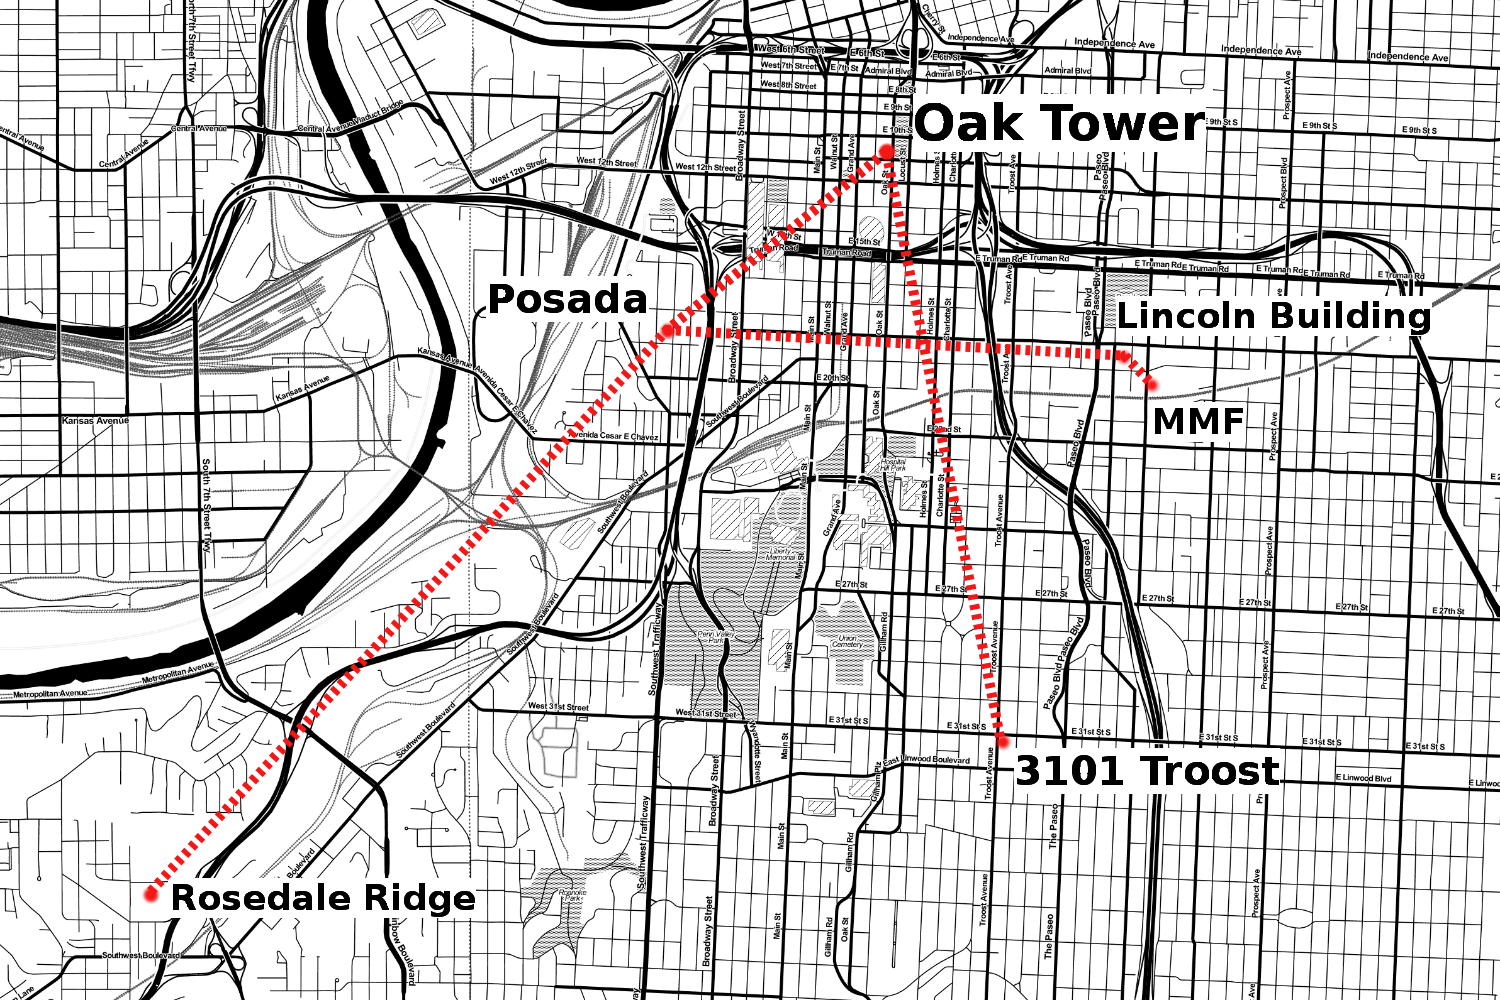
\includegraphics[width=3in]{es_toner_labelled.png}}
\fbox{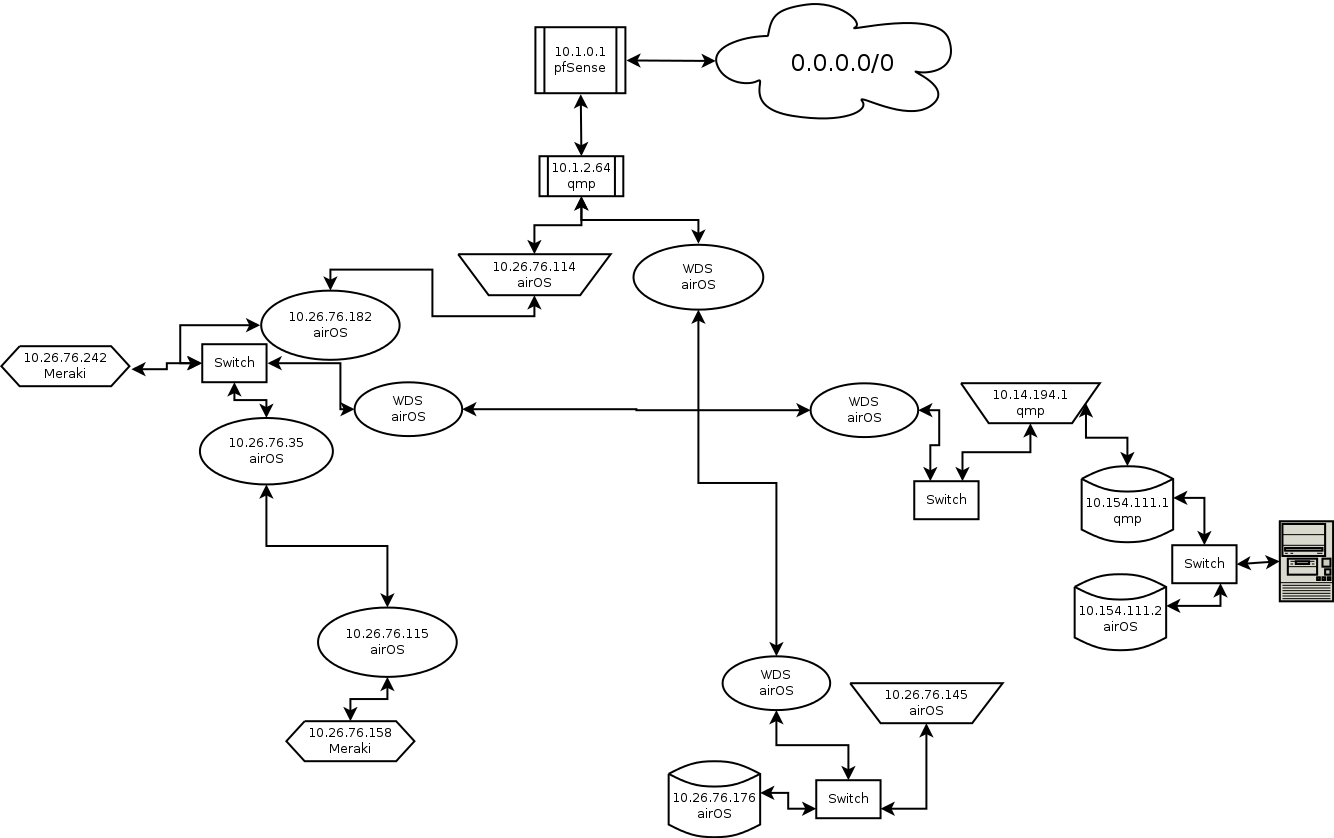
\includegraphics[width=5in]{Diagram1.png}}
\end{center}

While the figures above paint a decent picture of our current footprint, it is
equally important to understand the social and economic
infrastructure that supports these devices. The best way to understand the
network is to review the installations that are in place today:

\begin{description}
\item[Oak Tower]
Oak Tower, at 11\textsuperscript{th} and Oak, hosts the FreedomLink that currently serves as
KCFN's primary Internet gateway. The link is owned by Connecting
for Good, which purchases colocation, radio rights, and Internet service from
Joe's Datacenter on a monthly basis. \par
{\bf Technical Details:} This link consists of a single Dell server running
pfSense, connected to two Rocket M5's 
on the 27th floor via a Netgear 3800 running qmp. One Rocket is equipped with a
30 dBi dish antenna, while the other is equipped with a variable beam-width
sector antenna. Both radios shoot through storm 
windows to connect with the towers at 3101 Troost and Posada del Sol.

\item[Posada del Sol]
The FreedomTower at Posada del Sol, on the 1700 block of Summit Street in KC, MO
serves as an important distribution point in the network. The Mutual Musicians Foundation owns a dish that
connects to the Lincoln Building. Connecting for Good owns two dishes, with
one connecting to the sector antenna at Oak Tower, and the other connecting to the tower at
Rosedale Ridge. Six access points serve residents inside the building. The owner
of the building, Westside Housing, provides space to Connecting for Good and the
KCFN in exchange for network access. \par
{\bf Technical Details:} CFG owns two Rocket M5's with 30 dBi dish antennae. The
MMF owns a NanoBridge M365. All three radios are mounted to a 10'
non-penetrating mast atop the seven story building. Six Meraki access points ---
one on each floor --- distribute access throughout the building.  All three dishes, along with
one of the indoor access points, are linked to a five-port ToughSwitch and 
Uninterruptible Power Supply located in a utility closet on the seventh floor.

\item[Lincoln Building]
The FreedomTower at the Lincoln Building serves the area surrounding
18\textsuperscript{th}
\& Vine. Of the two radios at the Lincoln Building, one connects to Posada del
Sol, while the other anchors a neighborhood mesh. The tower is owned and operated by the Mutual Musician's Foundation, which
receives space from the Black Economic Union. \par
{\bf Technical Details} A NanoBridge M365 and Nanostation M5 are mounted to a 10' non-penetrating
mast atop the roof of the three story building. They are connected to a
TouchSwitch 
and UPS inside a utility closet on the third floor.

\item[Mutual Musicians Foundation] The MMF hosts a FreedomRelay, serving the
1800 block of Highland Ave, portions of 19th Street, and the Foundation itself.
In addition to a powerful mesh repeater, there is a dedicated media server, and a WiFi hotspot for the use
of musicians, administrators, and neighbors. \par
{\bf Technical Details:} A Rocket M5 with 10 dBi dual-omni, and a Bullet M2 with
9 dBi horizontal omni are attached to a 10'
hold-off mast anchored into roof cornice of the two story building. These radios
are attached to a ToughSwitch in the
first floor office via an alloy conduit anchored into exterior brick face. A
Dell XPS in the office runs Debian GNU/Linux, and is also attached to the
switch. 

\item[Rosedale Ridge]
The FreedomTower at Rosedale Ridge connects to Posada del Sol, and serves
residents of the complex via four access points. While the eqipment there is currently owned
by Connecting for Good, it is to be given to the complex owner, Yarco,
in December of 2013. \par
{\bf Technical Details:} A Rocket M5 with 30 dBi dish is mounted on a 10'
non-penetrating mast atop the three story building at the north of the complex.
Four Meraki access point in the courtyard distribute connectivity through the
complex.

\item[3101 Troost] The FreedomTower at 3101 Troost is jointly owned by
Reconciliation Services and Connecting for Good, and connects directly to the
FreedomLink at Oak Tower. In addition to one device dedicated to anchoring a
neighborhood mesh, there is a WiFi hot spot that serves the bus stop at
$31^{st}$ \& Troost. \par
{\bf Technical Details:} A Rocket M5 with 30 dBi dish is mounted on a railing
atop the five story building, and connects to Oak. A nearby non-penetrating boom
holds the Nanostation M2 Loco that lights up the bus stop. The Rocket M5 and
variable beam sector
that anchors the neighborhood network is mounted on a railing atop the belfry, one story up. 
\end{description}

